% 2008 年浙江卷文科第 15 题：球 O 的面上四点 A、B、C、D，DA⊥平面 ABC，AB⊥BC，
%   DA=AB=BC=√3。
% 来源 PDF：gaokaomath-src/普通高考/2008/2008浙江文.pdf
% SHA-256：751204c132deb2b2...
% 原页：2008浙江文.pdf 第 1 页（A3 三栏）第 2 栏，书页码 493。
% 重绘依据：D 在 A 的正上方（DA 竖直），B 在 A 左下、C 在 B 左侧，AB⊥BC；
%   可见棱 DA、DB、DC、AB、BC 实线，被遮挡的底面斜边 CA 虚线。
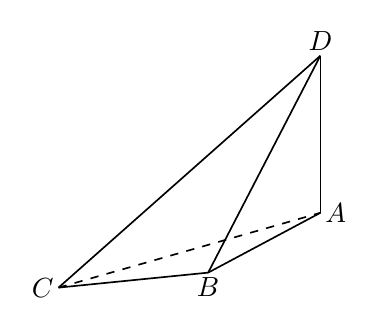
\begin{tikzpicture}[scale=0.95, semithick, every node/.style={inner sep=1.5pt}]
  \coordinate (D) at (5.0,4.7);
  \coordinate (A) at (5.0,2.6);
  \coordinate (B) at (3.5,1.8);
  \coordinate (C) at (1.5,1.6);

  \draw (D) -- (A);
  \draw (D) -- (B);
  \draw (D) -- (C);
  \draw (A) -- (B) -- (C);
  \draw[dashed] (C) -- (A);

  \node[above] at (D) {$D$};
  \node[right] at (A) {$A$};
  \node[below] at (B) {$B$};
  \node[left] at (C) {$C$};
\end{tikzpicture}
